% Tikzpicture Dichtungsring in schmaler Nut
        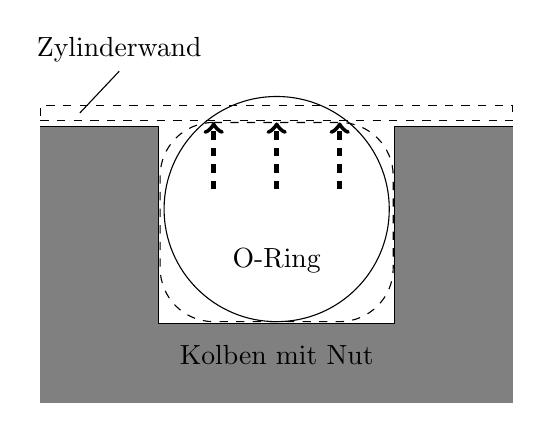
\begin{tikzpicture}
            \draw[gray, fill=gray] (.5,0) -- (2,0) -- (2,-2.5) -- (5,-2.5) -- (5,0) -- (6.5,0) -- (6.5,-3.5) -- (.5,-3.5) -- (.5,0);
            \draw (.5,0) -- (2,0) -- (2,-2.5) -- (5,-2.5) -- (5,0) -- (6.5,0);
            \draw (3.5,-1.05) circle (1.43);
            \draw[dashed] (.5,.07) -- (6.5,.07) -- (6.5,.27) -- (.5,.27) -- (.5,.07);
            \foreach \x in {2.7, 3.5, 4.3} \draw[ultra thick, ->, dashed] (\x,-.8) -- (\x,0.05);
            \draw[dashed] (2.7,.05) 
            -- (4.3,.05) 
            arc (90:0:.68) 
            -- (4.98,-1.8) 
            arc (0:-90:.68)
            -- (2.7,-2.48)
            arc (-90:-180:.68)
            -- (2.02,-.63)
            arc (-180:-270:.68);

            % Beschriftungen
            \draw (1.,.17) -- (1.5,.7) node[above] {Zylinderwand};
            \node at (3.5,-2.9)  {Kolben mit Nut};
            \node at (3.5,-1.7) {O-Ring};
        \end{tikzpicture}
